\documentclass[final]{fhnwreport}       %[mode] = draft or final
                                        %{class} = fhnwreport, article, 
                                        %          report, book, beamer, standalone

%%---Main Packages-----------------------------------------------------------------------
\usepackage[english, ngerman]{babel}	%Mul­tilin­gual sup­port for LaTeX
\usepackage[T1]{fontenc}				%Stan­dard pack­age for se­lect­ing font en­cod­ings
\usepackage[utf8]{inputenc}				%Ac­cept dif­fer­ent in­put en­cod­ings
\usepackage{lmodern}                    %The newer Font-Set
\usepackage{textcomp}					%LaTeX sup­port for the Text Com­pan­ion fonts
\usepackage{graphicx} 					%En­hanced sup­port for graph­ics
\usepackage{float}						%Im­proved in­ter­face for float­ing ob­jects
\usepackage{ifdraft}                    %Let you check if the doc is in draft mode

%%---Useful Packages---------------------------------------------------------------------
\usepackage[pdftex,dvipsnames]{xcolor}  %Driver-in­de­pen­dent color ex­ten­sions for LaTeX
\usepackage{csquotes}                   %Simpler quoting with \enquote{}
\usepackage{siunitx} 					%A com­pre­hen­sive (SI) units pack­age
\usepackage{listings}					%Type­set source code list­ings us­ing LaTeX
\usepackage[bottom]{footmisc}			%A range of foot­note op­tions
\usepackage{footnote}					%Im­prove on LaTeX's foot­note han­dling
\usepackage{verbatim}					%Reim­ple­men­ta­tion of and ex­ten­sions to LaTeX ver­ba­tim
\usepackage[textsize=footnotesize]{todonotes} %Mark­ing things to do in a LaTeX doc­u­ment

%%---Tikz Packages-----------------------------------------------------------------------
\usepackage{standalone}
\usepackage{tikz}
\usepackage{circuitikz}
\usetikzlibrary{arrows}
\usetikzlibrary{calc}
\usetikzlibrary{intersections}

%%---Math Packages-----------------------------------------------------------------------
\usepackage{amsmath}					%AMS math­e­mat­i­cal fa­cil­i­ties for LaTeX
%\usepackage{amssymb}					%Type­set­ting symbols (AMS style)
%\usepackage{array}						%Ex­tend­ing the ar­ray and tab­u­lar en­vi­ron­ments
%\usepackage{amsthm}					%Type­set­ting the­o­rems (AMS style)

%%---Table Packages----------------------------------------------------------------------
\usepackage{tabularx}					%Tab­u­lars with ad­justable-width columns
%\usepackage{longtable}
\usepackage{multirow}					%Create tab­u­lar cells span­ning mul­ti­ple rows
\usepackage{multicol}					%In­ter­mix sin­gle and mul­ti­ple columns

%%---PDF / Figure Packages---------------------------------------------------------------
\usepackage{pdfpages}					%In­clude PDF doc­u­ments in LaTeX
\usepackage{pdflscape}					%Make land­scape pages dis­play as land­scape
\usepackage{subfig}					    %Fig­ures di­vided into sub­fig­ures
\usepackage{placeins}                   % use \FloatBarrier to restrict float behind this place

%%---Other Packages----------------------------------------------------------------------
%\usepackage{xargs}                     %De­fine com­mands with many op­tional ar­gu­ments

%%---Bibliography------------------------------------------------------------------------
\usepackage[style=ieee,urldate=comp,backend=biber]{biblatex}
\addbibresource{literature/bibliography.bib}

%%---Main Settings-----------------------------------------------------------------------
\graphicspath{{./graphics/}}			%Defines the graphicspath
%\geometry{twoside=false}				    %twoside=false disables the "bookstyle"
\setlength{\marginparwidth}{2cm}
%\overfullrule=5em						%Creates a black rule if text goes over the margins => debugging


%%---User Definitions--------------------------------------------------------------------
%%Tabel-Definitions: (requires \usepackage{tabularx})
\newcolumntype{L}[1]{>{\raggedright\arraybackslash}p{#1}}    %column-width and alignment
\newcolumntype{C}[1]{>{\centering\arraybackslash}p{#1}}
\newcolumntype{R}[1]{>{\raggedleft\arraybackslash}p{#1}}

%%---Optional Package Settings-----------------------------------------------------------
%Listings-Settings: (requires \usepackage{listings}) => Example with Matlab Code
\lstset{language=Matlab,%
    basicstyle=\footnotesize\ttfamily,
    breaklines=false,%
    morekeywords={switch, case, otherwise},
    keywordstyle=\color{Blue},%
    tabsize=2,
    %morekeywords=[2]{1}, keywordstyle=[2]{\color{black}},
    identifierstyle=\color{Black},%
    stringstyle=\color{Purple},
    commentstyle=\color{Green},%
    showstringspaces=false,%without this there will be a symbol in the places where there is a space
    numbers=left,%
    numberstyle={\tiny \color{black}},% size of the numbers
    numbersep=9pt, % this defines how far the numbers are from the text
    %emph=[1]{word1, word2,...},emphstyle=[1]\color{red}
}				

%%---Projectspecific------------------------------------------------------------------------
\usepackage{pgfplots}	
%\usepackage{IEEEtrantools}	
%\usepackage{array}
%\usepackage{lipsum}
%\usepackage{etoolbox}
%\usepackage{setspace}
\usetikzlibrary{shapes,decorations.markings,backgrounds,patterns}
\usepackage[framed,numbered,autolinebreaks,useliterate]{mcode}

%%%
%%% For the SFGs
%%%
\tikzset{%
% Style of the node
    Node/.style={circle,thick,draw=black,inner sep=0, minimum size=0.15cm},
    Start/.style={draw=red},
    End/.style={draw=blue},
    Interm/.style={},
% Style of the node label
    NodeName/.style={font=\footnotesize,black, outer sep=1},
    NodeName n/.style={NodeName, above},
    NodeName s/.style={NodeName, below},
    NodeName e/.style={NodeName, right},
    NodeName w/.style={NodeName, left},
% Style of the branche label
    ArrowName/.style={font=\footnotesize,auto,outer sep=1},
    ArrowName n/.style={ArrowName, above},
    ArrowName s/.style={ArrowName, below},
    ArrowName e/.style={ArrowName, right},
    ArrowName w/.style={ArrowName, left},
% Style of the branch
    Connection/.style={thick},
    NodeBezier/.style={},
    ->-/.style={decoration={
        markings,
        %mark=at position #1 with {\arrow[scale=1.3,shorten >=1cm]{>}}},
        mark=at position #1 with {\draw[->,>=latex',ultra thick](0pt,0)--(4pt,0);}},
        postaction={decorate}},
    ->-/.default=0.50,
}

% Engineering

\makeatletter

\newif\ifpgfplots@scaled@x@ticks@engineering
\pgfplots@scaled@x@ticks@engineeringfalse
\newif\ifpgfplots@scaled@y@ticks@engineering
\pgfplots@scaled@y@ticks@engineeringfalse
\newif\ifpgfplots@scaled@z@ticks@engineering
\pgfplots@scaled@z@ticks@engineeringfalse

\pgfplotsset{
    scaled x ticks/engineering/.code=
        \pgfplots@scaled@x@ticks@engineeringtrue,
    scaled y ticks/engineering/.code=
        \pgfplots@scaled@y@ticks@engineeringtrue,
    scaled z ticks/engineering/.code=
        \pgfplots@scaled@y@ticks@engineeringtrue,
%    scaled ticks=engineering  % Uncomment this line if you want "engineering" to be on by default
}

\def\pgfplots@init@scaled@tick@for#1{%
    \global\def\pgfplots@glob@TMPa{0}%
    \expandafter\pgfplotslistcheckempty\csname pgfplots@prepared@tick@positions@major@#1\endcsname
    \ifpgfplotslistempty
        % we have no tick labels. Omit the tick scale label as well!
    \else
    \begingroup
    \ifcase\csname pgfplots@scaled@ticks@#1@choice\endcsname\relax
    % CASE 0 : scaled #1 ticks=false: do nothing here.
    \or
        % CASE 1 : scaled #1 ticks=true:
        %--------------------------------
        % the \pgfplots@xmin@unscaled@as@float  is set just before the data
        % scale transformation is initialised.
        %
        % The variables are empty if there is no datascale transformation.
        \expandafter\let\expandafter\pgfplots@cur@min@unscaled\csname pgfplots@#1min@unscaled@as@float\endcsname
        \expandafter\let\expandafter\pgfplots@cur@max@unscaled\csname pgfplots@#1max@unscaled@as@float\endcsname
        %
        \ifx\pgfplots@cur@min@unscaled\pgfutil@empty
            \edef\pgfplots@loc@TMPa{\csname pgfplots@#1min\endcsname}%
            \expandafter\pgfmathfloatparsenumber\expandafter{\pgfplots@loc@TMPa}%
            \let\pgfplots@cur@min@unscaled=\pgfmathresult
            \edef\pgfplots@loc@TMPa{\csname pgfplots@#1max\endcsname}%
            \expandafter\pgfmathfloatparsenumber\expandafter{\pgfplots@loc@TMPa}%
            \let\pgfplots@cur@max@unscaled=\pgfmathresult
        \fi
        %
        \expandafter\pgfmathfloat@decompose@E\pgfplots@cur@min@unscaled\relax\pgfmathfloat@a@E
        \expandafter\pgfmathfloat@decompose@E\pgfplots@cur@max@unscaled\relax\pgfmathfloat@b@E
        \pgfplots@init@scaled@tick@normalize@exponents
        \ifnum\pgfmathfloat@b@E<\pgfmathfloat@a@E
            \pgfmathfloat@b@E=\pgfmathfloat@a@E
        \fi
        \xdef\pgfplots@glob@TMPa{\pgfplots@scale@ticks@above@exponent}%
        \ifnum\pgfplots@glob@TMPa<\pgfmathfloat@b@E
            % ok, scale it:
            \expandafter\ifx % Check whether we're using engineering notation (restricting exponents to multiples of three)
                \csname ifpgfplots@scaled@#1@ticks@engineering\expandafter\endcsname
                \csname iftrue\endcsname
                    \divide\pgfmathfloat@b@E by 3
                    \multiply\pgfmathfloat@b@E by 3
            \fi
            \multiply\pgfmathfloat@b@E by-1
            \xdef\pgfplots@glob@TMPa{\the\pgfmathfloat@b@E}%
        \else
            \xdef\pgfplots@glob@TMPa{\pgfplots@scale@ticks@below@exponent}%
            \ifnum\pgfplots@glob@TMPa>\pgfmathfloat@b@E
                % ok, scale it:
                \expandafter\ifx % Check whether we're using engineering notation (restricting exponents to multiples of three)
                    \csname ifpgfplots@scaled@#1@ticks@engineering\expandafter\endcsname
                    \csname iftrue\endcsname
                        \advance\pgfmathfloat@b@E by -2
                        \divide\pgfmathfloat@b@E by 3
                        \multiply\pgfmathfloat@b@E by 3
                \fi
                \multiply\pgfmathfloat@b@E by-1
                \xdef\pgfplots@glob@TMPa{\the\pgfmathfloat@b@E}%
            \else
                % no scaling necessary:
                \xdef\pgfplots@glob@TMPa{0}%
            \fi
        \fi
    \or
        % CASE 2 : scaled #1 ticks=base 10:
        %--------------------------------
        \c@pgf@counta=\csname pgfplots@scaled@ticks@#1@arg\endcsname\relax
        %\multiply\c@pgf@counta by-1
        \xdef\pgfplots@glob@TMPa{\the\c@pgf@counta}%
    \or
        % CASE 3 : scaled #1 ticks=real:
        %--------------------------------
        \pgfmathfloatparsenumber{\csname pgfplots@scaled@ticks@#1@arg\endcsname}%
        \global\let\pgfplots@glob@TMPa=\pgfmathresult
    \or
        % CASE 4 : scaled #1 ticks=manual:
        \expandafter\global\expandafter\let\expandafter\pgfplots@glob@TMPa\csname pgfplots@scaled@ticks@#1@arg\endcsname
    \fi
    \endgroup
    \fi
    \expandafter\let\csname pgfplots@tick@scale@#1\endcsname=\pgfplots@glob@TMPa%
}
\makeatother			                %loads all packages, definitions and settings												
\title{Antennensimulationen in CST - Bericht hf1}          %Project Title
\author{Simon Zoller, Thomas Frei}          %Document Type => Technical Report, ...
\date{Windisch, \today}             %Place and Date


\begin{document}

%%---TITLEPAGE---------------------------------------------------------------------------
\selectlanguage{english}                %ngerman or english
\maketitle

\vspace*{-1cm}						    %compensates the space after the date line.
\vfill
%\begin{figure}[H]
%\centering
%\includegraphics[width=\linewidth]{titelbild.pdf}
%\end{figure}
\vfill

{
\renewcommand\arraystretch{2}
\begin{center}
\begin{tabular}{>{\bf}p{4cm} l}
Universität                &    Fachhochschule Nordwestschweiz\\
Studiengang                &    Elektro- und Informationstechnik\\
Autor   		           & 	Simon Zoller, Thomas Frei\\
Betreuer                   &    Christoph Wildfeuer und Peter Niklaus\\
Version                    &    1.0 %Normally not used!
\end{tabular}
\end{center}
}

\clearpage
			
%%---ABSTRACT----------------------------------------------------------------------------
\selectlanguage{english}				%ngerman or english
\thispagestyle{empty}
\include{sections/abstract}

%%---TABLE OF CONTENTS-------------------------------------------------------------------
\pagenumbering{Roman}		
\selectlanguage{english}				%ngerman or english
\tableofcontents
\clearpage

%%---TEXT--------------------------------------------------------------------------------
\pagenumbering{arabic}
\section{Einleitung}

Ein grosses Thema der Hochfrequenztechnik sind Antennen. Generell können Antennen als Leiter angesehen werden, welche identisch zur Leitungstheorie gelten. Jedoch gibt es viele verschiedene Ausführungen welche sich alle unterschiedlich verhalten. Während des Unterrichtes wurden keine Antennen angeschaut, weshalb sich mit diesem Bericht die Möglichkeit angeboten hat, diesen Teilbereich aufzuarbeiten. Hierfür wurden im Simulationsprogramm CST Messungen ausgewählter Antennen durchgeführt, welche sich vor allem auf die Direktivität der Antennen beziehen. Als Abschluss wurde noch eine Kleeblatt Antenne modelliert, mit welcher am Institut gearbeitet wird. Zu jeder Antenne wurde zuerst die Theorie behandelt und anschliessend die entsprechenden Simulationen durchgeführt. Die Theorie wurde nach dem Buch von K. Kark aufgearbeitet \cite{book}.
\section{Dipole}

Als erstes Thema werden Dipolantennen beschrieben. Dabei wird vor allem auf den Hertzschen Dipol eingegangen, welcher das Modell der Antenne vereinfacht.

\subsection{Hertzscher Dipol}

Eine Dipol Antenna kann als kurzer Linearstrahler beschrieben werden, wobei dessen länge $l \ll \lambda_0 /4$ beträgt. $\lambda_0$ beschreibt dabei die Wellenlänge, welche durch das Verhältnis der Lichtgeschwindigkeit zur Signalfrequenz $c_0/f$ beschreibt. 

xxx

Ein solcher Strahler ist in Abbildung xxx zu sehen, wobei $\underline{I}$ der komplexe Strom einer Sinusschwingung darstellt, welche konstant über die gesamte Länge schwingt. $\phi$ stellt den Winkel dar, welcher um die z-Achse rotiert und über die x- und y-Achse aufgespannt ist.$\theta$ hingegen rotiert um die x-Achse und wird über die y- und z-Achse aufgespannt. Für die Kugelkoordinaten bedeutet dies, dass mit den Restriktionen 

\begin{align}
&0 \leq \varphi \leq 2\pi\\
&0 \leq \vartheta \leq \pi
\end{align}

der gesamte Bereich des Koordinatensystems abgedeckt ist. Das durch den Strom induzierte Magnetfeld kann mit 

\begin{equation}
\underline{H}_0 = j\pi \frac{\underline{I}l}{{\lambda_0}^2}
\end{equation}

beschrieben werden, was für zwei Formeln für das magnetische und elektrische Feld liefert:

\begin{align}
\underline{H}_\varphi   &= \underline{H}_0 \sin \vartheta \frac{e^{-jk_0r}}{k_0r}\\
\underline{E}_\vartheta &= Z_0 \underline{H}_\varphi = Z_0 \underline{H}_0 \sin \vartheta \frac{e^{-jk_0r}}{k_0r}.
\end{align}

Hierbei beschreibt $r$ die Distanz des Punktes zu Ursprung und $k_0 = \omega \sqrt{\mu_0 \eta_0} = c_0/\omega$ die Wellenzahl im Vakuum beschreibt. Somit beschreibt die komplexe Exponentialfunktion die Ausbreitung der Welle, was mit der Theorie der Wellenleitern übereinstimmt. Im Nenner ist das Abklingen des Sinus zu erkennen, welches abhängig von der Distanz zum Ursprung und der Wellenzahl ist. xxx


\subsection{Richtdiagramm}

Ein wichtiges Diagramm für die Analyse von Antennen ist das Richtdiagramm. Mit diesem kann die Direktivität einer Antenne dargestellt werden, welche mitteilt, in welche Richtung wie viel der Leistung der Antenne abgestrahlt wird. Diese Analyse geschieht im Fernfeld, was bedeutet dass die Annahme $r \rightarrow \inf$ getroffen wird.

Im Fernfeld nimmt die Krümmung der sphärischen Phasenfront einer Kugelwelle immer weiter
ab. Für r   kann die Kugelwelle lokal durch eine homogene ebene Welle angenähert werden. Die transversalen Feldkomponenten werden phasengleich und es wird nur in radialer Richtung Wirkleistung transportiert, deren Winkelverteilung durch die Sendeantenne festgelegt ist.
Der Winkelabhängigkeit der Strahlung, d.h. der Strahlungsverteilung im Raum, kommt eine
große praktische Bedeutung zu. Von ihr hängt es ab, welcher Anteil der ausgestrahlten Leistung
für den eigentlichen Verwendungszweck ausgenutzt werden kann. Strahlung in oder Aufnahme
aus unerwünschten Richtungen erhöht die gegenseitigen Störungsmöglichkeiten. Bestimmte
Aufgaben verlangen vielfach auch eine ganz bestimmte Verteilung des Strahlungsfeldes. Einen
Überblick über die Verteilung der Strahlung in verschiedene Raumrichtungen liefert die Verteilung der Fernfeldstärke einer Antenne in Abhängigkeit von der Raumrichtung   , . 
\section{Gruppenantennen}\label{sec:gruppenantennen}
Der Dipol ist ein Rundstrahler, da die Strahlung keine bevorzugte Richtung in der Ebene senkrecht zur Antennenachse aufweist. Bei Punkt-zu-Punkt Verbindungen kann die Reichweite der Antenne bei unveränderter Energie erheblich vergrössert werden, wenn eine Richtwirkung vorhanden ist. Mit der Richtwirkung lässt sich der Störabstand verbessern, da mögliche Störquel-len durch die Richtcharakteristik zum Teil ausgeblendet werden. Eine gewünschte Richtwirkung kann durch Kombination zweier oder mehrerer Dipole mittels Interferenz der Feldstärken erzeugt werden.\\

Die folgenden Betrachtungen basieren auf dem linearen Superpositionsprinzip. Dies geht davon einer ungestörten Überlagerung der Strahlungsbeiträge aller Teilstrahler aus. Das Maximum des resultierenden Feldes befindet sich dort, wo die Felder der Einzelstrahler phasengleich schwingen. Die Felder der Einzelstrahler, die ausserhalb der Hauptstrahlungsrichtung sind, löschen sich gegenseitig mehr oder weniger aus. Die Richtwirkung kann mit diesen Faktoren beeinflusst werden.

\begin{itemize}
	\item Anzahl Strahler
	\item Anordnung der Strahler
	\item Stromamplitude der einzelnen Strahler
	\item Phasenverschiebung der einzelnen Strahler
\end{itemize}

In der Abbildung \ref{fig:gruppenantennen} sind drei unterschiedliche Formen von Gruppen aus Dipolantennen die sich für die Nachrichtenübertragung bewährt haben. 

\begin{figure}[H]
	\centering
	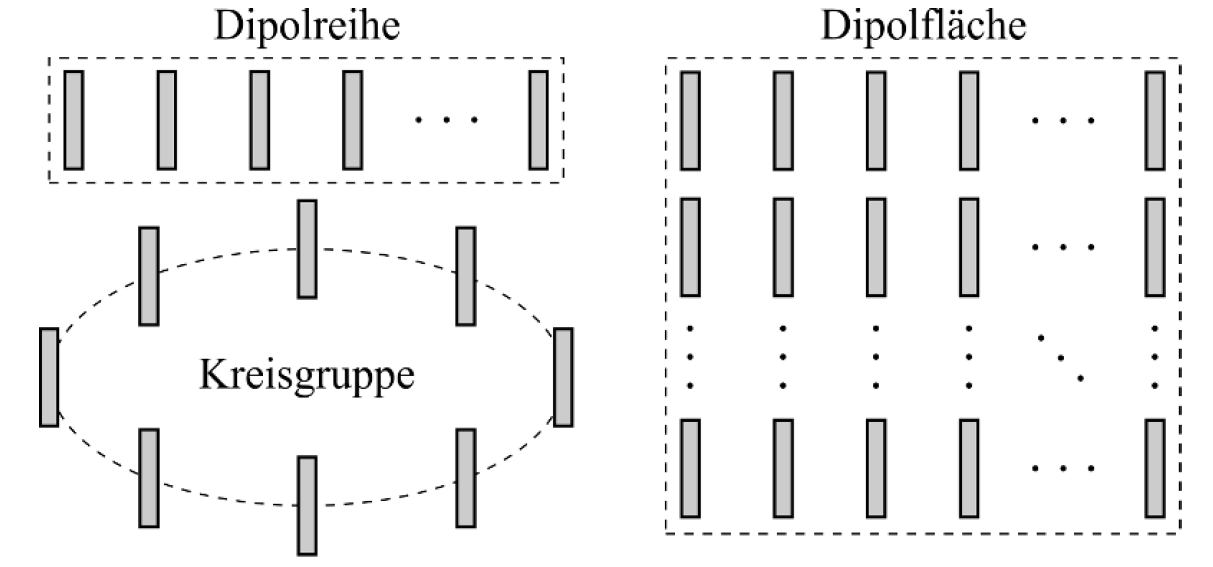
\includegraphics[width=0.75\linewidth]{gruppenantennen}
	\caption{Anordnung von Einzelstrahlern zu einer Antennengruppe.}\label{fig:gruppenantennen}
\end{figure}

Bei Strahlergruppen mit bauartgleichen Teilantennen in gleicher räumlicher Ausrichtung lässt sich das Fernfeld als Produkt von zwei Faktoren schreiben. Der erste Faktor ist die Einzelcharakteristik $ C_{E} $ und beschreibt das Fernfeld des einzelnen Antennenelementes. Die Gruppencharakteristik $ C_{Gr} $ ist der zweite Faktor. Er ist unabhängig von der Art des Einzelstrahlers und beschreibt das Zusammenwirken der Strahler. Unter der Voraussetzung dass die Entfernung des Aufpunktes im Fernfeld gross gegen die räumlichen Abmessungen des Antennensystems aus mehreren Einzelstrahlern und gross gegen die Wellenlänge $ \lambda_{0} $ so können die beiden Faktoren multipliziert werden. Dies ergibt die nachfolgende Formel.

\begin{equation}
C_{ges}=C_{Gr}C_{E}
\end{equation}


\subsection{Querstrahler}\label{sec:querstrahler}

Der Querstrahler gehört zu den linearen Gruppenstrahler und ist eine Dipolzeile, welche in der Abbildung \ref{fig:dipolzeile} dargestellt ist. Bei dieser Gruppe stehen die Dipole senkrecht zur Standlinie (y-Achse).\\

Beim Querstrahler ist die Gruppencharakteristik rotationssymmetrisch zur Gruppenachse. Sie entsteht indem alle Einzelstrahler gleichphasig $ \delta = 0$ erregt werden. Denn dann sind in der Mittelsenkrechten zur Gruppenachse ihre sämtlichen Feldanteile in Phase. Zusätzlich muss der Elementabstand $ a < \lambda_{0} $ sein, damit der Hauptanteil der Energie senkrecht zur Gruppenachse in einen scheibenförmigen Sektor ausgestrahlt wird und weitere Hauptkeulen nicht auftreten können. 

\begin{figure}[H]
	\centering
	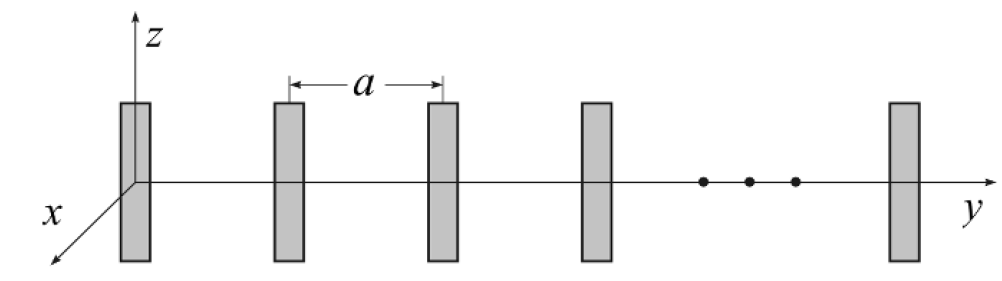
\includegraphics[width=0.75\linewidth]{dipolzeile}
	\caption{Anordnung von baugleichen, äquidistanten Einzelstrahlern zu einer Horizontaler Dipolzeile.}\label{fig:dipolzeile}
\end{figure}

\subsection{Simulation}

Für die Simulation ist eine querstrahlende Dipolzeile mit zwei Einzelstrahler, wie in der Abbildung \ref{fig:querstrahler} aufgebaut worden. Der Dipolabstand beträgt $ a = 2\lambda_{0} $. Dieser führt bei einfacher Speisung zu einer guten Querabstrahlung bei kleinen Nebenkeulen. 

\begin{figure}[!ht]
	\centering
	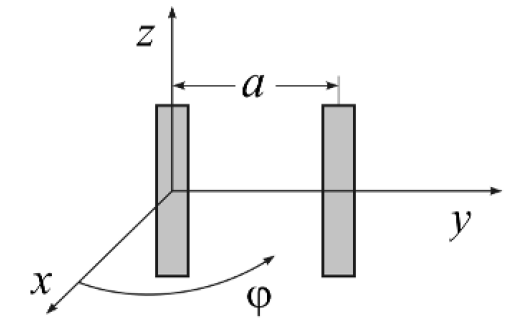
\includegraphics[width=0.5\linewidth]{querstrahler}
	\caption{Aufbau des Querstrahlers.}\label{fig:querstrahler}
\end{figure}

Die Gruppencharakteristik für zwei Strahlerelemente lässt sich mit der Formel einer linearen Gruppe wie folgt berechnen:

\begin{equation}
C_{Gr}(\vartheta,\varphi) = \left|  \cos \left( \dfrac{\sin(N u/2)}{N \sin(u/2)}  \right) \right| = \left|  \cos \left( \dfrac{\sin(u)}{2 \sin(u/2)}  \right) \right|.
\end{equation}

Diese Formel lässt sich vereinfachen und erhält dieses Resultat:

\begin{equation}
C_{Gr}(\vartheta,\varphi) = \left|  \cos \left( \dfrac{k_{0} a}{2} \sin \vartheta \sin\varphi \right) \right|.
\end{equation} 

Das horizontale Richtdiagramm erhält man für $ \vartheta = \pi / 2 $:

\begin{equation}
C_{Gr}^{H}(\varphi) = \left|  \cos \left( \dfrac{\pi a}{\lambda_{0}} \sin \varphi \right) \right|.
\end{equation} 

\begin{figure}[!ht]
	\centering
	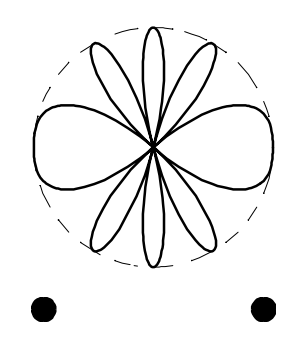
\includegraphics[width=0.4\linewidth]{2Lambda.png}
	\caption{Direktivität des Antennenarrays mit einem Abstand von $2\lambda_0$.}\label{fig:2Lambda}
\end{figure}

In Abbildung \ref{fig:2Lambda} ist das Richtdiagramm für zwei Dipole mit dem Abstand $2\lambda_0$ zu sehen. Dies ist das erwünschte Resultat der Simulation.

\newpage

\begin{figure}[!ht]
	\centering
	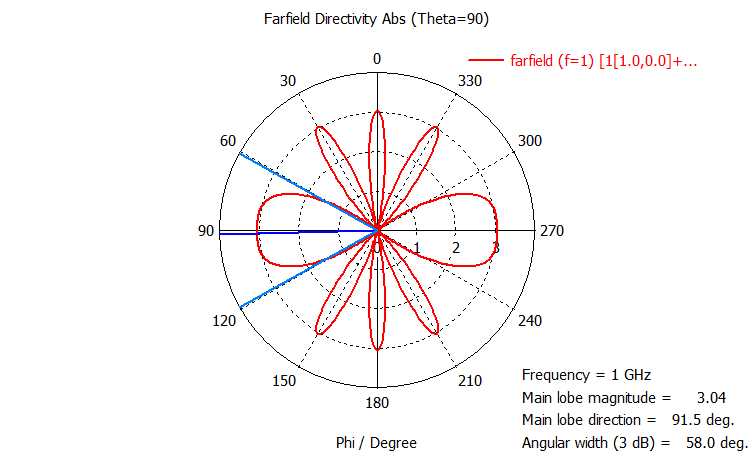
\includegraphics[width=\linewidth]{Array.png}
	\caption{Simulation des Antennenarrays mit $a = 2\lambda_0$.}\label{fig:Array}
\end{figure}

In der Abbildung \ref{fig:Array} ist das Richtdiagramm grafisch dargestellt. Die Anzahl der Nebenkeulen und auch die Form des Richtdiagrammes stimmen mit dem erwarteten Plot überein, weshalb die Simulation als erfolgreich angesehen werden kann. Was jedoch beachtet werden muss, ist dass durch die Abstrahlcharakteristik das Richtdiagramm bei einem konstanten Winkel von $\vartheta$ ausgewertet werden muss, welcher \SI{90}{\degree} beträgt.

%%---BIBLIOGRAPHY------------------------------------------------------------------------
{\sloppypar
\printbibliography[heading=bibintoc]
\label{sec:lit}
}

%%---APPENDIX----------------------------------------------------------------------------
%\include{sections/appendix}

%%---NOTES for DEBUG---------------------------------------------------------------------
\ifdraft{%Do this only if mode=draft
%%requires \usepackage{todonotes})
\newpage
\listoftodos[\section{Todo-Notes}]
\clearpage
}
{%Do this only if mode=final 
}
\end{document}
